\chapter{Machine Learning Modeling Review}
\label{ch2}

PyTorch reference \cite{NEURIPS2019_9015}.

\section{Fundamentals of Training and Testing}
\begin{figure}[h!]
	\centering
		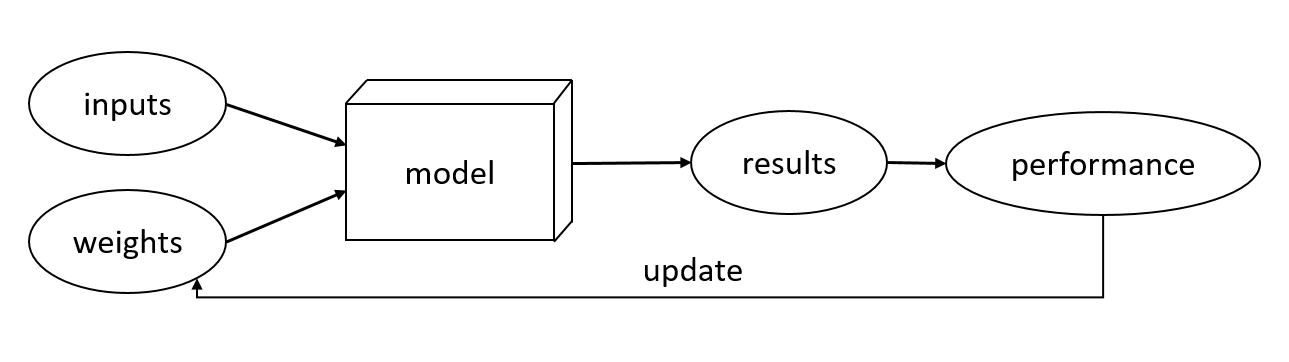
\includegraphics[width=0.99\textwidth]
		{training_process.png}
		\hfill
		\caption{Simple example of machine learning model training .}
		\label{fig:simple_model_training}
\end{figure}

\begin{figure}[h!]
	\centering
	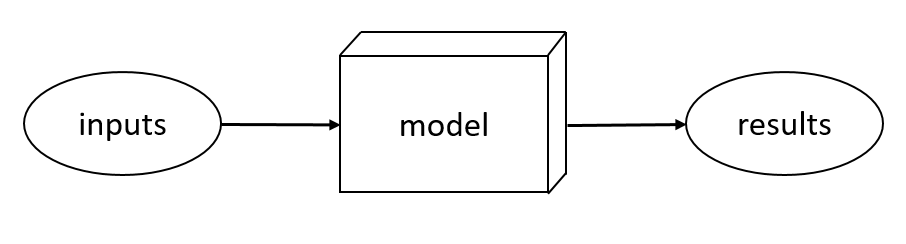
\includegraphics[width=0.99\textwidth]
	{testing_process.png}
	\hfill
	\caption{Simple example of machine learning model testing.}
	\label{fig:simple_model_testing}
\end{figure}

%\begin{figure}[h!]
%	\centering
%	\subfloat[Training\label{fig:simple_model_training_testing_a}]{
%		\includegraphics[width=0.99\textwidth]
%		{training_process.png}
%	}
%	\hfill
%	\subfloat[Testing\label{fig:simple_model_training_testing_b}]{
%		\includegraphics[width=0.99\textwidth]
%		{testing_process.png}
%	}
%	\hfill
%	\caption{Simple example of machine learning model training and testing.}
%	\label{fig:simple_model_training_testing}
%\end{figure}

\section{MLP and RNN Architectures}
\subsection{MLP}
\begin{equation} \label{eq:MLP}
	y = \sigma \left(xA^{T} + b\right)
\end{equation}
where (I think) $x$ is the input, $A^{T}$ is the transformation matrix, and $b$ is the bias.

\subsection{RNN}
For each element in the input sequence, each layer computes the following function:
\begin{equation} \label{eq:RNN}
	h_{t} = \tanh\left(W_{ih}x_{t} + b_{ih} + W_{hh}h_{\left(t-1\right)} + b_{hh}\right)
\end{equation}
where $h_{t}$ is the hidden state at time $t$, $x_{t}$ is the input at time $t$, and $h_{\left(t-1\right)}$ is the hidden state of the previous layer at time $t-1$ or the initial state at time 0 (zero).

\subsection{GRU}
For each element in the input sequence, each layer computes the following function:
\begin{align}
	r_{t} &= \sigma\left(W_{ir}x_{t} + b_{ir} + W_{hr}h_{\left(t-1\right)} + b_{hr}\right) \label{eq:GRU1} \\
	z_{t} &= \sigma\left(W_{iz}x_{t} + b_{iz} + W_{hz}h_{\left(t-1\right)} + b_{hz}\right) \label{eq:GRU2} \\
	n_{t} &= \tanh\left(W_{in}x_{t} + b_{in} + r_{t} \odot \left(W_{hn}h_{\left(t-1\right)} b_{hn}\right)\right) \label{eq:GRU3} \\
	h_{t} &= \left(1 - z_{t}\right) \odot n_{t} + z_{t} \odot h_{\left(t-1\right)} \label{eq:GRU4}
\end{align}
where $h_{t}$ is the hidden state at time $t$, $x_{t}$ is the input at time $t$, $h_{\left(t-1\right)}$ is the hidden state of the layer at time $t-1$ or the initial hidden state at time 0 (zero), and $r_{t}$, $z_{t}$, and $n_{t}$ are the reset, update, and new gates, respectively. $\sigma$ is the sigmoid function, and $\odot$ is the Hadamard (element-wise) product. Equations \ref{eq:GRU1}, \ref{eq:GRU2}, \ref{eq:GRU3}, \ref{eq:GRU4}.

\subsection{LSTM}
For each element in the input sequence, each layer computes the following function:
\begin{align}
	i_{t} &= \sigma\left(W_{ii}x_{t} + b_{ii} + W_{hi}h_{\left(t-1\right)} + b_{hi}\right) \label{eq:LSTM1} \\
	f_{t} &= \sigma\left(W_{if}x_{t} + b_{if} + W_{hf}h_{\left(t-1\right)} + b_{hf}\right) \label{eq:LSTM2} \\
	g_{t} &= \tanh\left(W_{ig}x_{t} + b_{ig} + W_{hg}h_{\left(t-1\right)} + b_{hg}\right) \label{eq:LSTM3} \\
	o_{t} &= \sigma\left(W_{io}x_{t} + b_{io} + W_{ho}h_{\left(t-1\right)} + b_{ho}\right) \label{eq:LSTM4} \\
	c_{t} &= f_{t} \odot c_{\left(t-1\right)} + i_{t} \odot g_{t} \label{eq:LSTM5} \\
	h_{t} &= o_{t} \odot \tanh\left(c_{t}\right) \label{eq:LSTM6}
\end{align}
where $h_{t}$ is the hidden state at time $t$, $c_{t}$ is the cell state at time $t$, $x_{t}$ is the input at time $t$, $h_{\left(t-1\right)}$ is the hidden state of the layer at time $t-1$ or the initial state at time 0 (zero), and $i_{t}$, $f_{t}$, $g_{t}$, and $o_{t}$ are the input, forget, cell, and output gates, respectively. $\sigma$ is the sigmoid function, and $\odot$ is the Hadamard (element-wise) product. Equations \ref{eq:LSTM1}, \ref{eq:LSTM2}, \ref{eq:LSTM3}, \ref{eq:LSTM4}, \ref{eq:LSTM5}, \ref{eq:LSTM6}.

\section{Optimization and Loss Function}

\section{Chapter Summary?}